\documentclass{article}
% translate with >> pdflatex -shell-escape <file>

% This file is an extract of the PGFPLOTS manual, copyright by Christian Feuersaenger.
% 
% Feel free to use it as long as you cite the pgfplots manual properly.
%
% See
%   http://pgfplots.sourceforge.net/pgfplots.pdf
% for the complete manual.
%
% Any required input files (for <plot table> or <plot file> or the table package) can be downloaded
% at
% http://www.ctan.org/tex-archive/graphics/pgf/contrib/pgfplots/doc/latex/
% and
% http://www.ctan.org/tex-archive/graphics/pgf/contrib/pgfplots/doc/latex/plotdata/

\usepackage{pgfplots}
\pgfplotsset{compat=newest}

\pagestyle{empty}

\begin{document}
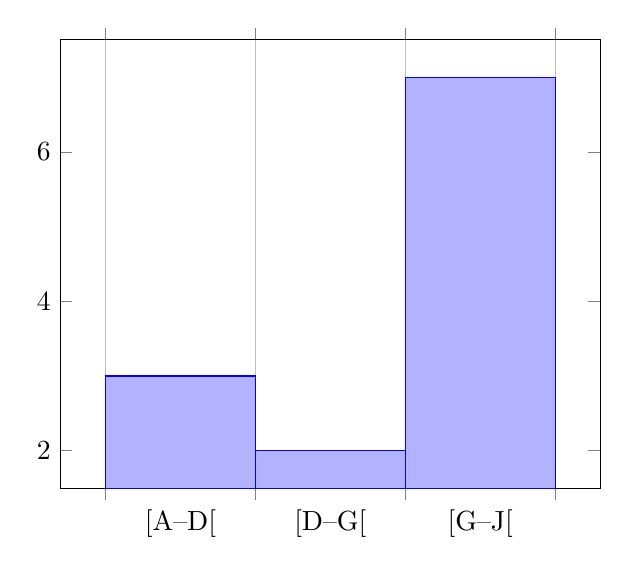
\begin{tikzpicture}
\begin{axis}[
  ybar interval,
  hist/symbolic coords={A,B,C,D,E,F,G,H,I,J},
  xticklabel={[\tick--\nexttick[},
]
    \addplot+[hist={bins=3}]
        table[row sep=\\,y index=0] {
        data\\
		A\\ B\\ A\\ D\\ F\\ J\\
		G\\ J\\ I\\ H\\ I\\ I\\
    };
\end{axis}
\end{tikzpicture}
\end{document}
